\documentclass[11pt]{beamer}
\usetheme{simple}
\setbeamertemplate{footline}{} 
\usepackage{tikz}

\usepackage{pgfplots}
\usepackage{amsmath, amssymb, amsthm}   
\pgfplotsset{
        % declare the function you want to plot so you can reuse it easily later
        /pgf/declare function={
            T1(\u)=ln(0.5*(-2*\u+sqrt(4+4*\u^2)));
            T0(\u)=ln(0.5*(2*\u+sqrt(44+4*\u^2)));     
            U0(\u)=\u-1;
            T12(\u)=ln(-1-2*\u);
        },
        % define style to use for the plot to draw only ticks at `\myxlist'
        % (the plot should be invisible)
        my ticks/.style={
            samples at={\myxlist},
            mark=none,
            draw=none,
%            only marks,     % <-- uncomment me to show the data points
        },
every non boxed y axis/.append style={y axis line style=-}
    }
%\pgfplotsset{ every non boxed y axis/.append style={y axis line style=-}}
\setbeamertemplate{navigation symbols}{}
\begin{document}
\begin{frame}


\tikzset{every picture/.style={line width=0.75pt}} %set default line width to 0.75pt        

\begin{tikzpicture}[x=0.75pt,y=0.75pt,yscale=-.75,xscale=.75]
%uncomment if require: \path (0,465.3999996185303); %set diagram left start at 0, and has height of 465.3999996185303



%Shape: Axis 2D [id:dp11877989343343409] 
\draw  (53.3,382.93) -- (560.88,382.93)(104.06,36.6) -- (104.06,421.41) (553.88,377.93) -- (560.88,382.93) -- (553.88,387.93) (99.06,43.6) -- (104.06,36.6) -- (109.06,43.6)  ;
%Straight Lines [id:da35120644981115934] 
\draw [color={rgb, 255:red, 74; green, 74; blue, 74 }  ,draw opacity=1 ][line width=1.5]    (102.98,252) -- (470.42,383) ;

%Curve Lines [id:da6451900492142217] 
\draw [color={rgb, 255:red, 74; green, 144; blue, 226 }  ,draw opacity=0.99 ][line width=2.25]    (208.29,24) .. controls (302.8,365.8) and (291.8,359.6) .. (585.8,356.6) ;

% Text Node
\draw (376.65,325.56) node   {$x^{*}$};

%dot x^*
\draw [shift={(363.23,344)}, rotate = 0] [color={rgb, 255:red, 0; green, 0; blue, 0 }  ][fill={rgb, 255:red, 0; green, 0; blue, 0 }  ][line width=0.75]      (0,0) circle [x radius= 3.35, y radius= 3.35]   ;

% Text Node
\draw (571.61,402.33) node   {$x_{1}$};
% Text Node
\draw (69.16,44.56) node   {$x_{2}$};
% Text Node
\draw (131.61,282) node   {$B( r_{1})$};

\only<2,3,4>{
%Straight Lines [id:da7950102729434785] 
\draw [color={rgb, 255:red, 245; green, 166; blue, 35 }  ,draw opacity=1 ][line width=1.5]    (104.4,54.4) -- (303.4,382.4) ;

% Text Node
\draw (246.31,318) node   {$m$};

% Text Node
\draw (136.61,154) node   {$\textcolor[rgb]{0.96,0.65,0.14}{B( r_{2})}$};

%dot m
\draw    (257,307.6) ;
\draw [shift={(257,307.6)}, rotate = 0] [color={rgb, 255:red, 0; green, 0; blue, 0 }  ][fill={rgb, 255:red, 0; green, 0; blue, 0 }  ][line width=0.75]      (0, 0) circle [x radius= 3.35, y radius= 3.35]   ;}






\only<3,4>{%Straight Lines [id:da9164907770746624] 
\draw [color={rgb, 255:red, 0; green, 0; blue, 0 }  ,draw opacity=1 ][line width=1.5]  [dash pattern={on 5.63pt off 4.5pt}]  (144.4,31.4) -- (351.4,383.4) ;

%dot x^h [id:da623174012393656] 
\draw    (292.8,284.8) ;
\draw [shift={(292.8,284.8)}, rotate = 0] [color={rgb, 255:red, 0; green, 0; blue, 0 }  ][fill={rgb, 255:red, 0; green, 0; blue, 0 }  ][line width=0.75]      (0, 0) circle [x radius= 3.35, y radius= 3.35]   ;

%Curve Lines [id:da7465497407939561] 
\draw [color={rgb, 255:red, 208; green, 2; blue, 27 }  ,draw opacity=1 ]   (363.23,344) .. controls (358.28,293.37) and (328.12,263.5) .. (294.35,283.84) ;
\draw [shift={(292.8,284.8)}, rotate = 327.15999999999997] [fill={rgb, 255:red, 208; green, 2; blue, 27 }  ,fill opacity=1 ][line width=0.75]  [draw opacity=0] (8.93,-4.29) -- (0,0) -- (8.93,4.29) -- cycle    ;}





\only<4>{


%Curve Lines [id:da18724695995674012] 
\draw [color={rgb, 255:red, 74; green, 144; blue, 226 }  ,draw opacity=0.99 ][line width=2.25]    (152.76,20) .. controls (237.1,346) and (248.8,372.6) .. (592.8,371.6) ;

%Straight Lines [id:da5040887194933186] 
\draw    (363.23,344) ;

%dot x^** [id:da5639887056281057] 
\draw    (231.48,263) ;
\draw [shift={(231.48,263)}, rotate = 0] [color={rgb, 255:red, 0; green, 0; blue, 0 }  ][fill={rgb, 255:red, 0; green, 0; blue, 0 }  ][line width=0.75]      (0, 0) circle [x radius= 3.35, y radius= 3.35]   ;





%%%% effect lines

\draw    (293,415.6) -- (362,416.6) ;
\draw [shift={(362,416.6)}, rotate = 180.83] [color={rgb, 255:red, 0; green, 0; blue, 0 }  ][line width=0.75]    (0,5.59) -- (0,-5.59)   ;
\draw [shift={(293,415.6)}, rotate = 180.83] [color={rgb, 255:red, 0; green, 0; blue, 0 }  ][line width=0.75]    (0,5.59) -- (0,-5.59)   ;

%Straight Lines [id:da4561185972885533] 
\draw  [dash pattern={on 0.84pt off 2.51pt}]  (231.48,263) -- (231.48,406.6) ;


%Straight Lines [id:da7973470416027963] 
\draw  [dash pattern={on 0.84pt off 2.51pt}]  (292.8,284.8) -- (292.8,430.6) ;


%Straight Lines [id:da6192414642962101] 
\draw  [dash pattern={on 0.84pt off 2.51pt}]  (363.23,344) -- (363,432.6) ;

%Straight Lines [id:da964413909902704] 
\draw    (231,406.6) -- (293,406.6) ;
\draw [shift={(293,406.6)}, rotate = 180] [color={rgb, 255:red, 0; green, 0; blue, 0 }  ][line width=0.75]    (0,5.59) -- (0,-5.59)   ;
\draw [shift={(231,406.6)}, rotate = 180] [color={rgb, 255:red, 0; green, 0; blue, 0 }  ][line width=0.75]    (0,5.59) -- (0,-5.59)   ;
%%% end effect lines



%Curve Lines [id:da898754754978262] 
\draw [color={rgb, 255:red, 208; green, 2; blue, 27 }  ,draw opacity=1 ]   (292.8,284.8) .. controls (274.38,263.04) and (258.64,253) .. (233.06,262.4) ;
\draw [shift={(231.48,263)}, rotate = 338.59000000000003] [fill={rgb, 255:red, 208; green, 2; blue, 27 }  ,fill opacity=1 ][line width=0.75]  [draw opacity=0] (8.93,-4.29) -- (0,0) -- (8.93,4.29) -- cycle    ;




% Text Node
\draw (131.61,282) node   {$B( r_{1})$};
% Text Node
\draw (136.61,154) node   {$\textcolor[rgb]{0.96,0.65,0.14}{B( r_{2})}$};




% Text Node
\draw (212.65,264.56) node   {$x^{**}$};
% Text Node
\draw (329,404) node  [align=left] {{\tiny subst. eff.}};
% Text Node
\draw (261,395) node  [align=left] {{\tiny income. eff.}};
% Text Node
\draw (363,442.6) node   {$x^{*}_{1}$};
% Text Node
\draw (292.8,443.6) node   {$x^{h}_{1}$};
% Text Node
\draw (231.65,425.56) node   {$x^{**}_{1}$};}



\end{tikzpicture}

\end{frame}\end{document}